\begin{minipage}[b]{0.7\textwidth}

\begin{Exercise}[label  = rotierendes 3-Körper-Problem, difficulty = 3, label = cmrot, origin = {XX. IPhO 1989}, title = Starrer Körper]
	Drei (nicht-kolineare) Massen $m_i$ ($i \in \{1,2,3\}$) an Punkten $P_i$ wechselwirken ausschließlich über durch ihre Gravitationskraft. Die durch die drei Punkte aufgespannte Ebene sei $\nu$, und die dazu senkrecht stehende Rotationsachse $\sigma$. Welche Bedingungen müssen die drei Seitenlängen des Dreiecks $\Delta P_1P_2P_3$ erfüllen, sodass dieses sich nicht verändert, also wie ein starrer Körper um $\sigma$ rotiert?
\end{Exercise}
\end{minipage}
\begin{minipage}[b]{0.3\textwidth}
	\centering
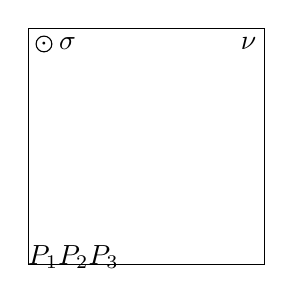
\begin{tikzpicture}
	\draw (0,0) rectangle (3,3);
	\node at (2.8,2.8) {$\nu$};
	\draw (0.2,2.8) circle (0.1);
	\node at (0.2,2.8) {$\cdot$};
	\node at (0.5,2.8) {$\sigma$};
	
	\tkzDefPoint(0.5,0.5){A}
	\tkzDefPoint(2.7,0.3){B}
	\tkzDefPoint(1.2,2.5){C}
	
	\tkzDrawPoints(A,B,C)
	\tkzLabelPoint[above](A){$P_1$}
	\tkzLabelPoint[above](B){$P_2$}
	\tkzLabelPoint[right](C){$P_3$}
	
	
\end{tikzpicture}
\end{minipage}